First thing we had to do in TRITIUM experiment was to choose the optimal fiber length at which the signal from the tritium events is optimized. To make this decision we have to take into account that, on the one hand, long fibers are interesting because the efficiency of our detector is proporcional to the active area, which is proporcional to the fiber length but, on the other hand, in long fibers, scintillation photons will need to be reflected in the fiber walls more times to be driven to its ends, where it will be detected by photosensors and this is a problem because we lose photons in each reflection, deteriorating the detector signal.

Several simulations were performed using Geant4 \cite{Geant4WebPage}, a particle and nuclear physics simulation package based on C++, to quantify, between other things, the importance of this effect and to allow us to choose the optimal fiber length. The results of this simulations will be shown in the section \ref{sec:ResultsSimulations}, where they will be discussed. In these simulations it has been seen that it is preferable to work with short fiber (figure \ref{}). The fiber length, which has been chosen for the tritium prototypes developed in Valencia, is $20~\cm$ and the fiber length used in each study will be named in the appropriate section, but it will be close to this value.

Saint Gobain's commercial fibers are 1 meter long, so first thing we had to do was cut the scintillation fibers before using it. It is very important to introduce strict requirements on the cutting quality of the fiber ends since it will greatly affect the transmission of photons and, thus, the efficiency of TRITIUM monitor. This cut must be perpendicular to the fiber and very low uncertainty in the length of the fiber, both requeriments are mandatory to achieve a good coupling with the surface of the photosensor. It is also important that its final state must be as clean as possible, that is, without cracks or deformations because it will contribute to internal reflections, losing photons and, thus, reducing the tritium signal.

Cutting the end faces of polymer fibers is one of current challenges. There are many different techniques such as milling, laser cutting, focused-ion-beam, blade cutting, etc. Due to its simplicity, we have focused on blade cleaving. %I had these references in the "Smooth end face termination of microstructured, graded-index, and step-index polymer optical fibers" paper

Many commercial devices based on blade cleaving, such as the one provided by thorlabs with a diamond tipped blade \cite{DiamondThorlabs} or others similar to the guillotine designed for industrial fiber optics \cite{GuillotineIFO}, were tested in a extensive study done but with unsuccessful results \cite{TFGAlberto}. As can be seen in figures \ref{fig:BadCutsOfFibers}, it presents deformations, cracks or imperfections so the technics considered in this study don't overcome the requirements imposed.

\begin{figure}[htbp]
 \centering
  \subfloat[Fiber end deformation.]{
   \label{subfig:FiberEndDeformation}
    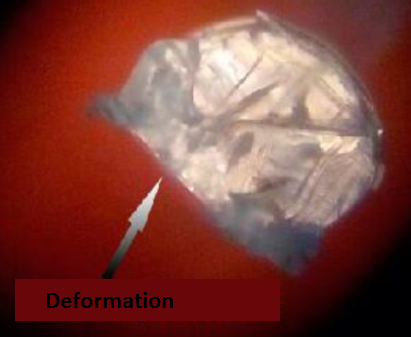
\includegraphics[width=0.5\textwidth]{4ResearchAndDevelopments/41Fibers/DeformationFiberEnds.png}}
    %\newline
  \subfloat[Fiber end cracks.]{
   \label{subfig:FiberEndCracks}
    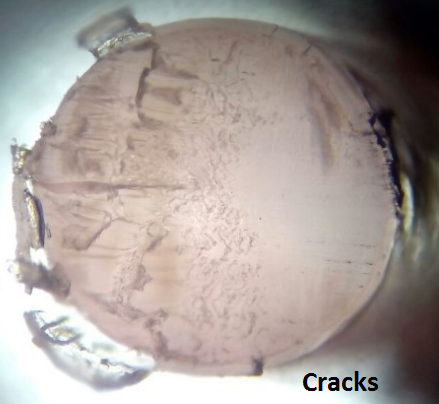
\includegraphics[width=0.45\textwidth]{4ResearchAndDevelopments/41Fibers/CracksEndFibers.png}}
 \caption{Unsuccessful results of using commercial techniques to cut fibers.}
 \label{fig:BadCutsOfFibers}
\end{figure}

The microscope model PB 4161 from EUROMEX company or the Digital Microscope from Jiusion company, shown in figures \ref{fig:Microscopes}, were used to check the results in the fiber ends.

\begin{figure}[htbp]
 \centering
  \subfloat[EUROMEX microscope]{
   \label{subfig:EUROMEXMicroscope}
    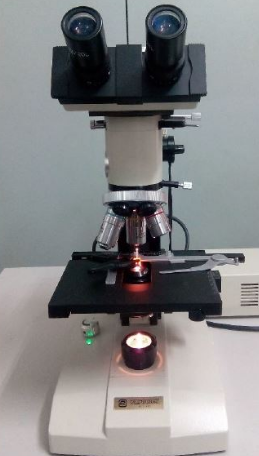
\includegraphics[width=0.25\textwidth]{4ResearchAndDevelopments/41Fibers/EuromexMicroscope.png}}
    %\newline
  \subfloat[Jiusion microscope]{
   \label{subfig:JiusionMicroscope}
    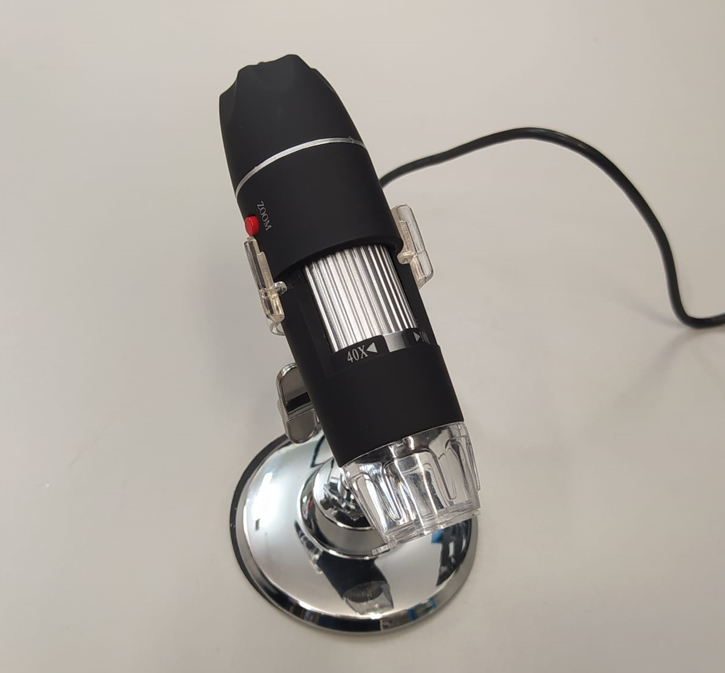
\includegraphics[width=0.45\textwidth]{4ResearchAndDevelopments/41Fibers/JiusionMicroscope.png}}
 \caption{Microscopes used to check the results.}
 \label{fig:Microscopes}
\end{figure}

Because commercial devices don't work for our scintillating fibers, we had to design, build and test our own cutting device, which is shown in figure \ref{fig:CuttingTRITIUMDevice}.

\begin{figure}[htbp]
 \centering
  \subfloat[TRITIUM Cutting device]{
   \label{subfig:CuttingDevice1}
    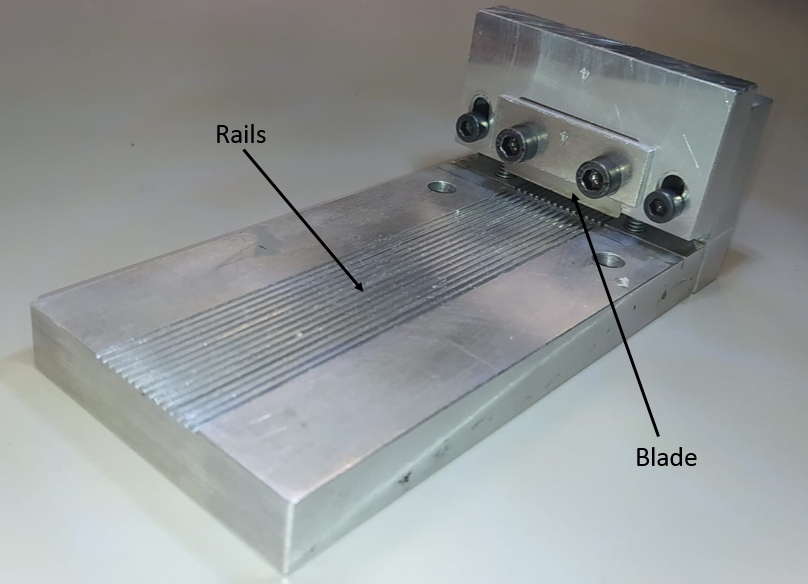
\includegraphics[width=0.4\textwidth]{4ResearchAndDevelopments/41Fibers/CuttingDevice1.png}}
    %\newline
  \subfloat[TRITIUM Cutting device]{
   \label{subfig:CuttingDevice2}
    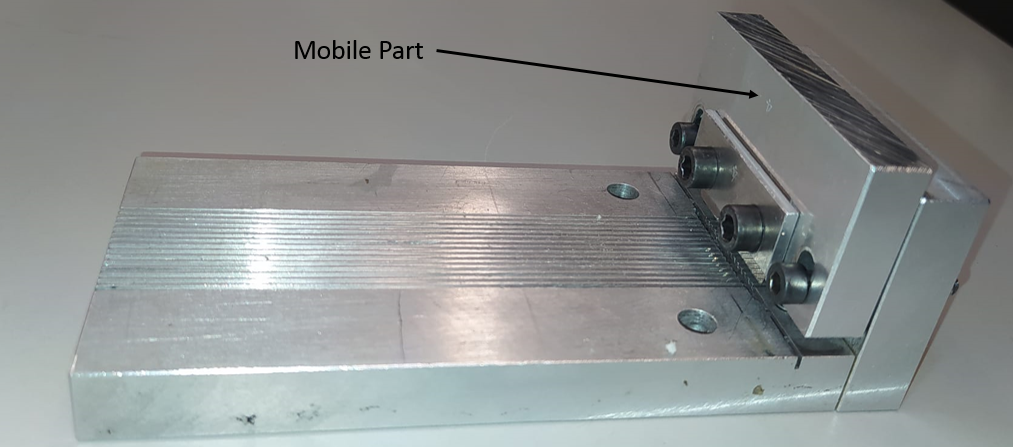
\includegraphics[width=0.55\textwidth]{4ResearchAndDevelopments/41Fibers/CuttingDevice2.png}}
    \newline
    \subfloat[Additional piece of TRITIUM cutting device]{
   \label{subfig:AdditionalPieceCuttingDevice}
    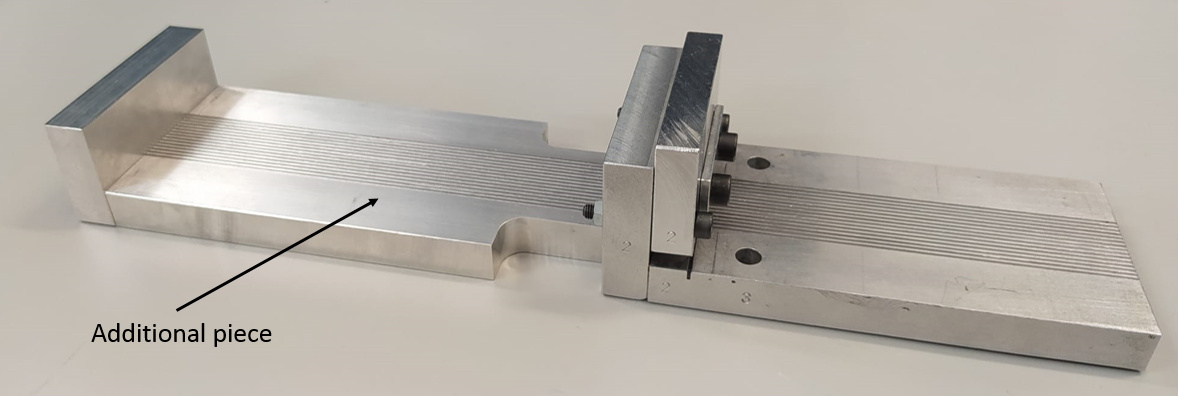
\includegraphics[width=0.6\textwidth]{4ResearchAndDevelopments/41Fibers/AdditionalPieceCuttingDevice.png}}
 \caption{Cutting device developed in the TRITIUM experiment and additional part to make precise measurements of fiber length.}
 \label{fig:CuttingTRITIUMDevice}
\end{figure}

It consists of fourteen rails where the fibers will be fixed and a thin blade, fixed on a mobile piece, perpendicular to the fibers, with which we can be sure of achieving a perpendicular cut, which is one of the requirements imposed.

The blade used is the typical commercial razor blade, whose thickness is $0.1~\mm$, which is the thickness with which we obtain the best results and it was positioned with a slight inclination, $5\degree$, with respect to the horizontal axis since it has been seen in several studies that this helps to obtain a less aggressive and cleaner cut  \cite{AngleBlade}, \cite{TemperatureBlade}.

Therefore, as can be seen in the figure \ref{subfig:CutFiberEnd}, with this device we obtain fiber ends without breaks or deformation overcoming another imposed requirement.

Another important parameter that can affect the cutting quality of the fiber ends is the temperature of both, either the fiber or the blade. It has been tested in a study in which both were subjected to different temperatures from room temperature (25 degrees) to 110 degrees \cite{TFGAlberto}. No significant conclusions were obtained in the temperature study, so we work at room temperature to facilitate the cutting technic.

To obtain a low enough length uncertainty, which is the last requirement we must overcome, we designed and built an additional piece, shown in figure \ref{subfig:AdditionalPieceCuttingDevice}, which is used to measure the fiber. With this piece we achieve an uncertainty in the measurement of less than 1 millimeter.

With the designed cutting fiber device we have exceeded all requirements imposed, obtaining a cut fiber end whose quality is high enough to ensure that it will affect the transmission of light as little as possible.

In the figure \ref{subfig:CutFiberEnd}, which shows the fiber end after cutting process with TRITIUM cutting device, you can see a slightly darkened part at the bottom of the fiber, which is an inevitable effect of the cutting process. To repair this imperfection, a polishing process developed by thorlabs is included \cite{DiamondThorlabs}. 

This polishing process consists of using five different polishing papers, with a decreasing grain size, whose diameters are $30~\mu\meter$, $20~\mu\meter$, $12~\mu\meter$, $5~\mu\meter$ and $0.3~\mu\meter$ respectively, in which we describe movements in the shape of 8 for two minutes (approximately 120 movements). 

The result obtained with this polishing process is shown in figure \ref{subfig:PolishFiberEnd}. In the figure \ref{fig:ResultofPolishingProcess}, the quality of both fiber ends, before and after polishing process, can be compared. There, we can see that the darkened part has completely disappeared. 

\begin{figure}[htbp]
 \centering
  \subfloat[Fiber end after cutting with Tritium device.]{
   \label{subfig:CutFiberEnd}
    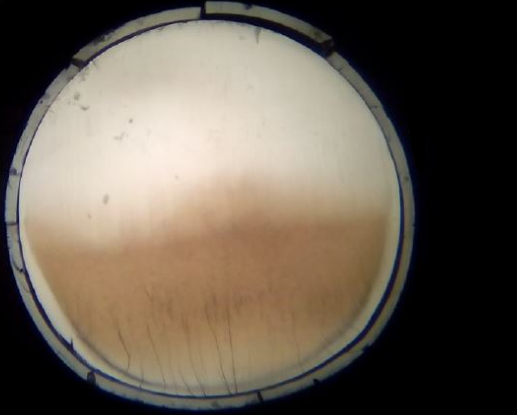
\includegraphics[width=0.5\textwidth]{4ResearchAndDevelopments/41Fibers/CutEndFiberGood.png}}
    %\newline
  \subfloat[Fiber end after cutting and polishing.]{
   \label{subfig:PolishFiberEnd}
    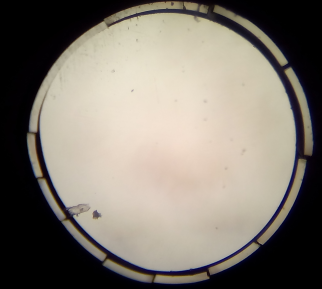
\includegraphics[width=0.45\textwidth]{4ResearchAndDevelopments/41Fibers/CutAndPolishedFiberEnd.png}}
 \caption{Result of the polishing process. a) Fiber end after cutting with TRITIUM devices b) Fiber end after cutting with TRITIUM devices and polishing with Thorlabs technic.}
 \label{fig:ResultofPolishingProcess}
\end{figure}

The end of the cut fiber is completely clear after cutting and polishing, without any damage or imperfection, so both tasks, cutting and polishing, will make up the conditioning process developed for each fiber before any study or its introduction into the TRITIUM detector.